\documentclass[11pt,a4paper]{article}
\usepackage{jheppub}
\usepackage{slashed}
\usepackage{amsthm}

\usepackage{mathtools}  

% BOXES
\usepackage{color}
\definecolor{myblue}{rgb}{.8, .8, 1}
\usepackage{empheq}

\usepackage{physics} %Im in imaginary part

\usepackage{slashed}


\newlength\mytemplen
\newsavebox\mytempbox

\makeatletter
\newcommand\mybluebox{%
    \@ifnextchar[%]
       {\@mybluebox}%
       {\@mybluebox[0pt]}}

\def\@mybluebox[#1]{%
    \@ifnextchar[%]
       {\@@mybluebox[#1]}%
       {\@@mybluebox[#1][0pt]}}

\def\@@mybluebox[#1][#2]#3{
    \sbox\mytempbox{#3}%
    \mytemplen\ht\mytempbox
    \advance\mytemplen #1\relax
    \ht\mytempbox\mytemplen
    \mytemplen\dp\mytempbox
    \advance\mytemplen #2\relax
    \dp\mytempbox\mytemplen
    \colorbox{myblue}{\hspace{1em}\usebox{\mytempbox}\hspace{1em}}}

\makeatother
%%%%%%%%%%%5

\newcommand*\diff{\mathop{}\!\mathrm{d}}
\newcommand*\Diff[1]{\mathop{}\!\mathrm{d^#1}}

%%%%%%%%%%%%%%%%%%%%%%%%%%%%%% User specified LaTeX commands.


%%%%%%%%%%%%%%%%%%%%%%%%%%%%%%%%%%%%%%%%%%%%%%%%%%%%%%%%%%%%%%%%%%%%%%%%%%%%
%%%%%%%%%%%%%%%%%%%%%%%% MAIN BODY OF THE ARTICLE %%%%%%%%%%%%%%%%%%%%%%%%%%
%%%%%%%%%%%%%%%%%%%%%%%%%%%%%%%%%%%%%%%%%%%%%%%%%%%%%%%%%%%%%%%%%%%%%%%%%%%%

%\subheader{13.10.2015}

\title{$e^+ e^-$ Scattering to Hadrons Notes}

\author[a]{Dirk Hornung}

\affiliation[a]{Institut de F\'\i sica d’Altes Energies (IFAE), The Barcelona 
                Institute of Science and Technology,\\ Campus UAB,
                08193 Bellaterra (Barcelona) Spain}

\emailAdd{dirkhornung91@gmail.com}


\abstract{Abstract...}%

\keywords{Keywords...}

\let\conj

\begin{document}
\maketitle

% 
\section{Non-degenerated Time Independent Perturbation Theory}
Let $E^{(0)}$ and $| n^{(0)} \rangle$ be the known eigenvalue and eigenvector of
\begin{equation}
	H^{(0)} | n^{(0)} \rangle = E_n^{(0)} | n^{(0)} \rangle.
\end{equation}
Introducing a small correction (perturbation) $V$ we want to find the approximated solution of 
\begin{equation}
	\label{perturbedSchroedinger}
	(H^{(0)} +  \lambda V)| n \rangle = E_n | n \rangle,
\end{equation}
where we introduced $\lambda \in [0, 1]$ to keep track of the strength of the perturbation:
\begin{align}
	\lambda &= 0 \quad \to \quad \text{unperturbed case} \\
	\lambda &= 1 \quad \to \quad \text{perturbed case}.
\end{align}
By defining the so-called energy shift
\begin{equation}
	\Delta_n \equiv E_n - E_n^{(0)}
\end{equation}
we can write
\begin{equation}
	(E_n^{(0)} - H^{(0)}) | n \rangle = ( \Delta_n + E_n^{(0)}) | n \rangle.
\end{equation}
For finding a solution we want to invert $(E_n^{(0)} - H^{(0)})$ which is in general not always well defined
\begin{equation} 
	\frac{1}{E_n^{(0)} - H^{(0)})} | n^{(0)} \rangle = \frac{1}{0} | n^{(0)} \rangle, 
\end{equation}
thus we define the complementary projector
\begin{equation}
	\phi_n \equiv 1 - | n^{(0)} \rangle \langle n^{(0)} | =  \sum_{k \neq n} | k^{(0)} \rangle \langle k^{(0)} |.
\end{equation}
Multiplicating the complementary projector from the left side yields
\begin{equation}
	| n \rangle = \frac{\phi_n (\lambda V - \Delta_n ) }{E_n^{(0)} - H^{(0)}} | n\rangle, 
\end{equation}
where we used 
\begin{align}
	&\phi_n (\lambda V - \Delta_n ) | n \rangle = (\lambda V - \Delta_n) | n \rangle, \\
	\text{because:} \quad &\langle n^{(0)} | E_n^{(0)} - H^{(0)} | n \rangle = \langle n^{(0)} \lambda V - \Delta_n | n \rangle = 0.
\end{align}
In the limit $\lambda \to 1$ this result turns out to be zero so we'll add $c_n(\lambda) | n^{(0)} \rangle$ to $| n \rangle$
\begin{equation}
	| n \rangle = c_n(\lambda) | n^{(0)} + \frac{\phi_n (\lambda V - \Delta_n ) }{E_n^{(0)} - H^{(0)}} | n\rangle.
\end{equation}
We can do this, because $c_n(\lambda) | n^{(0)} \rangle$ is like adding a zero term
\begin{equation}
	(E_n^{(0)} - H^{(0)}) | n^{(0)} \rangle = 0.
\end{equation}
Furthermore regarding the limit and defining a new normalization (for convenience) gives us
\begin{equation}
	\lim_{\lambda \to 0} c_n(\lambda) = 1, \quad c_n(\lambda) = \langle n^{(0)} | n \rangle = 1
\end{equation}
and thus the eigenkets and the energy shift are given as
\begin{align}
	\label{schroedingerEigenket}
	&| n \rangle = |  n^{(0)}\rangle + \frac{\phi_n (\lambda V - \Delta_n ) }{E_n^{(0)} - H^{(0)}} | n\rangle \\
	&\Delta_n = \lambda \langle n^{(0)} | V | n \rangle, \quad \text{because:} \langle n^{(0)} | \lambda V - \Delta_n | n \rangle = 0.
\end{align}
Expanding in terms of $\lambda$ yields
\begin{align}
	|n\rangle &= |n^{(0)} \rangle + \lambda |n^{(1)} \rangle + \lambda^2 |n^{(2)} \rangle + \cdots \\
	\Delta_n &= \lambda \Delta_n^{(1)} + \lambda^2 \Delta_n^{(2)} + \cdots
\end{align}
So by comparing $\lambda$ order by order we get for the energy shift
\begin{align}
	\mathcal{O}(\lambda^1): \qquad \Delta_n^{(1)} &= \langle n^{(0)} | V | n^{(0)} \rangle \\
	\mathcal{O}(\lambda^2): \qquad \Delta_n^{(2)} &= \langle n^{(0)} | V | n^{(1)} \rangle \\
	& \vdots \\
	\mathcal{O}(\lambda^N): \qquad \Delta_n^{(1)} &= \langle n^{(0)} | V | n^{(N-1)} \rangle
\end{align}.
Thus finding the eigenkets $|n^{(N-1)}\rangle$ is neccesary for calculating the energy perturbations
\begin{align}
	| n \rangle &= |  n^{(0)} + \frac{\phi_n (\lambda V - \Delta_n ) }{E_n^{(0)} - H^{(0)}} | n\rangle \\
			&= |n^{(0)} \rangle + \frac{\phi_n}{E_n^{(0)} - H_n^{(0)}} ( \lambda V - \lambda \Delta_n^{(1)} - \lambda^2 \Delta_n^{(2)} - \cdots) \times ( |n^{(0)} \rangle + \lambda | n^{(1)} \rangle + \cdots ), 
\end{align}
where we expanded both sides of \ref{schroedingerEigenket}. This being done we can now compare each order of lamba. Starting with the first order eigenket
\begin{align}
	\mathcal{O}(\lambda^1): \qquad &|n^{(1)}\rangle = \frac{\phi_n}{E_n^{(0)} + H_n^{(0)}} (V - \Delta_n^{(1)} ) | n^{(0)} \rangle, \\
	\text{because} \quad &\phi_n \Delta_n^{(1)} | n^{(0)} \rangle = 0.
\end{align}
With this in mind we easily get the expression for 
\begin{equation}
	\Delta_n^{(2)} = \langle n^{(0)} | V | n^{(1)} \rangle = \langle n^{(0)} | V \frac{\phi_n}{E_n^{(0)} - H_n^{(0)}} V | n^{(0)} \rangle,
\end{equation}
with which we can calculate the following order in $|n\rangle$
\begin{align}
	\mathcal{O}(\lambda^2) |n^{(2)} \rangle &= \frac{\phi_n}{E_n^{(0)} - H_n^{(0)}} (V | n^{(1)} \rangle - \Delta_n^{(1)} | n^{(1)} \rangle - \underbrace{\Delta_n^{(2)} | n^{(0)} \rangle}_{0} ) \\
	&= \frac{\phi_n}{E_n^{(0)} - H_n^{(0)}} V \frac{\phi_n}{E_n^{(0)} - H_n^{(0)}} | n^{(0)}\rangle \\
	&- \frac{\phi_n}{E_n^{(0)} - H_n^{(0)}} \langle n^{(0)}|V|n^{(0)}\rangle \frac{\phi_n}{E_n^{(0)} - H_n^{(0)}} V | n^{(0)}\rangle
\end{align}
and so on and so forth. By defining
\begin{equation}
	V_{nk} = \langle n^{(0)}|V|k^{(0)}\rangle
\end{equation}
we can sum up the final result of non-degenerated time-independent PT as
\begin{align}
	\Delta_n &= E_n - E_n^{(0)} \\
	&= \lambda \Delta^{(1)} + \lambda^2 \Delta^{(2)} + \cdots \\
	&= \lambda V_{nn} + \lambda^2 \sum_{k \neq n} \frac{|V_{nk}|^2}{E_n^{(0)} - E_k^{(0)}} + \cdots \\
	|n\rangle &= |n^{(0)}\rangle + \lambda |n^{(1)}\rangle + \lambda^2|n^{(2)}\rangle + \cdots \\
	&= |n^{(0)}\rangle + \lambda \sum_{k\neq n} \frac{|k^{(0)}\rangle V_{kn}}{E_n^{(0)}-E_k^{(0)}} \\
	&+ \lambda^2 \left( \sum_{k\neq n}\sum_{l\neq n} \frac{|k^{(0)}\rangle V_{kl}V_{ln}}{(E_n^{(0)}-E_k^{(0)})(E_n^{(0)}-E_l^{(0)})} - \sum_{k\neq n} \frac{V_{nn}V_{kk}}{(E_n^{(0)} - E_k^{(0)})^2} \right).
\end{align}



\section{Feynman Propagator}
In this section we want to derive the Feynman propagator for scalors $\Pi(p)$ defined as the Greens function within the time ordered product of two scalar fields $\phi(x)$ and $\phi(y)$
\begin{equation}
	\langle 0 | T \{ \phi(x) \phi(y) \} | 0 \rangle = \int \frac{d^4}{(2\pi)^4} \exp^{i p (x-y)} \Pi(p).
\end{equation}
The general approach for getting an expression for the free propagator will be to calculate the time ordered product of the two free fields and compare the result with the above definition. 
As starting point we will use the free scalar field
\begin{equation}
	\phi_0(\vec x, t) = \int \frac{d^3 k}{(2\pi)^3} \frac{1}{\sqrt{2 w_k}} (a_k \exp^{i \vec k \vec x} + a_k^\dagger \exp^{-\vec k \vec x} )
\end{equation},
where $\omega_k = k_0 = \sqrt{m^2 + \vec k^2}$. Thus forming the free field non time ordered product we get
\begin{equation}
	\langle 0 | \phi(x_1) \phi(x_2) | 0 \rangle = \int \frac{d^3 k_1}{(2\pi)^3} \int \frac{d^3 k_2}{(2\pi)^3} \frac{1}{\sqrt{\omega_{k_1}}}\frac{1}{\sqrt{\omega_{k_2}}}  e^{i(k_1 x_1-  k_2 x_2)} \langle 0 | (a_{k_1}  a_{k_2}^\dagger | 0 \rangle
\end{equation}, where the the missing ladder operator summands within the vacuum are zero. The momentum of the created particle needs to be annihilated at a later time. Consequently the product of the annihilation and creation operator within the vacuum gives us
\begin{equation}
	\langle 0 | (a_{k_1}  a_{k_2}^\dagger | 0 \rangle = \delta^3(k_1 - k_2)
\end{equation},
so we can evaluate one of the two integrals
\begin{align}
	\langle 0 | \phi(x_1) \phi(x_2) | 0 \rangle &= \int \frac{d^3 k_1}{(2\pi)^3} \int \frac{d^3 k_2}{(2\pi)^3} \frac{1}{\sqrt{\omega_{k_1}}}\frac{1}{\sqrt{\omega_{k_2}}}  e^{i(k_1 x_1-  k_2 x_2)}  \delta^3(k_1 - k_2)  \\
	&= \int \frac{d^3 k}{(2\pi)^3} \frac{1}{2\omega_k} e^{i k(x_1-x_2)}
\end{align}.
Now we can write the time ordered field products as product of the Heaviside-function $\Theta(x)$
\begin{align}
	\langle 0 | T\{\phi(x_1) \phi(x_2) \} | 0 \rangle &= \int \frac{d^3 k}{(2\pi)^3} \frac{1}{2 \omega_k} [ e^{ik(x_1 - x_2)}\Theta(t_1-t_2) + e^{ik(x_2-x_1)} \Theta(t_2 - t_1)]  \\
	&= \int \frac{d^3 k}{(2\pi)^3} \frac{1}{2 \omega_k} [ e^{i\vec k (\vec x_1-\vec x_2)}e^{-i \omega_k \tau} \Theta(\tau) + e^{i\vec k ( \vec x_1 - \vec x_2)} e^{i \omega_k \tau} \Theta(- \tau)]  \\
	&= \int \frac{d^3 k}{(2\pi)^3} \frac{1}{2 \omega_k}  e^{-i\vec k (\vec x_1-\vec x_2)}[e^{-i \omega_k \tau} \Theta(\tau) + e^{i \omega_k \tau} \Theta(- \tau)]  
\end{align},
where we subsituted $\tau = t_1 - t_2$ in the second line and $k \to -k$ in the third line.
The time dependent Heaviside-functions can be rewritten with two contour integrals
\begin{equation}
	e^{-i \omega_k \tau} \Theta(\tau) + e^{i \omega_k \tau} \Theta(- \tau) = \lim_{\epsilon \to 0} \frac{- 2 \omega_k}{2\pi i} \int_{-\infty}^{\infty} \frac{d \omega}{\omega^2 - \omega_k^2 + i \epsilon} e^{i \omega \tau},
\end{equation}
which we will check now.
To derive this identity we first separate out the poles with partial fractions
\begin{align}
	\frac{1}{\omega^2 - \omega_k^2 + i\epsilon} &= \frac{1}{\omega - (\omega_k - i\epsilon)} \frac{1}{(\omega - (-\omega_k + i\epsilon)} \\
	&= \frac{1}{2 \omega_k}  \left [\frac{1}{\omega - (\omega_k - i\epsilon)} - \frac{1}{\omega - (\omega_k + i\epsilon)}  \right ].
\end{align}
Applying the Residue theorem
\begin{equation}
	\oint_C f(z) dz = \int_{-a}^{a} f(z) dz  + \int_{arc} f(z) dz = 2 \pi i \sum_{k=1}^n I(C, a_k) Res(f, a_k),
\end{equation}
(check wiki for details). Our line integral has two residuum
\begin{equation}
	\underset{\omega = \omega_k + i\epsilon}{Res} (f(\omega)) = e^{i \omega_k \tau}, \qquad \underset{\omega = -\omega_k - i\epsilon}{Res} (f(\omega)) =   e^{-i \omega_k \tau}
\end{equation}
yielding
\begin{align}
	\lim_{\epsilon \to 0} \frac{- 2 \omega_k}{2\pi i} \int_{-\infty}^{\infty} \frac{d \omega}{\omega^2 - \omega_k^2 + i \epsilon} e^{i \omega \tau} &= - \frac{2 \omega_k}{2 \pi i} \frac{1}{2 \omega_k} \int_{-\infty}^{\infty} \left[ \frac{d\omega e^{i\omega \tau}}{\omega - (\omega_k - i\epsilon)} + \frac{d \omega e^{i\omega\tau}}{\omega - (\omega + i\epsilon)} \right] \\
	&=  e^{-i\omega_k \tau} \Theta(\tau) + e^{i \omega_k \tau} \Theta(\tau). \qquad \square
\end{align}
So finally we have for the Feynman propagator
\begin{align}
	\langle 0 | T \{ \phi(x_1) \phi(x_2) \} | 0 \rangle &= \int \frac{d^3}{(2\pi)^3} \frac{1}{\omega_k} e^{i \vec k(\vec x_1 \vec x_2)} \left[ \frac{-2 \omega_k}{2 \pi i} \int \frac{d\omega}{\omega^2 - \omega_k + i\epsilon} e^{i\omega \tau} \right] \\
	&= \int\int \frac{d^3k d\omega}{(2 \pi)^4} \frac{i}{\omega^2 - \omega_k^2 + i\epsilon} e^{i [\vec k (\vec x_1 - \vec x_2) + \omega \tau]} \\
	&= \int \frac{d^4 k}{(2\pi)^4}\frac{i}{w^2 - m^2 - k^2 + i\epsilon} e^{ik(x_1 - x_2)} \\
	&= \int \frac{d^4 k}{(2\pi)^4} \frac{i}{k^2 - m^2 + i\epsilon} e^{ik (x_1 - x_2)}
\end{align}

\section{Photon Propagator}\label{sec:photonPropagator}
In this section we will derive the Photon propagator
\begin{equation}
	\langle 0 | T\{ A^\mu (x) A^\nu (y) \} | 0 \rangle = i \int \frac{d^4 p}{(2 \pi)^4} e^{ip(x-y)} \Pi^{\mu\nu}(p).
\end{equation}
Starting by the Maxwell Lagrangian
\begin{equation}
	\mathcal{L} = - \frac{1}{4} F_{\mu\nu}^2 - A_\mu J_\mu, \quad \text{with} \quad F_{\mu\nu} = \partial_\mu A_\nu - \partial_\nu A_\mu,
\end{equation}
we can apply the Euler-Lagrange equation
\begin{align}
	\frac{\partial \mathcal{L}}{\partial A_\alpha} - \partial_\beta \frac{\partial \mathcal{L}}{\partial(\partial_\beta A_\alpha)} &= -J_\alpha + \frac{2}{4} \partial_\beta [(\delta_\beta^\mu \delta_\alpha^\nu - \delta_\beta^\nu \delta_\alpha^\mu) (\partial_\mu A_\nu - \partial_\nu A_\mu) ] \\
	&= -J_\alpha + \frac{1}{2} \partial_\beta \underbrace{(\partial_\beta A_\alpha - \partial_\alpha A_\beta - \partial_\alpha A_\beta + \partial_\beta A_\alpha)}_{2F_{\beta\alpha}} \\
	\Rightarrow \partial_\mu F_{\mu\nu} &= \partial_\mu(\partial_\nu A_\nu - \partial_\nu A_\mu) =  J_\nu
\end{align}
or in momentum Space
\begin{equation}
	(-k^2 g_{\mu\nu} + k_\mu k_\nu) A_\mu = J_\nu.
\end{equation}
We would like to write $A_\mu = \Pi_{\mu\nu} J_\nu$, meaning that we have to invert $(-p^2 g_{\mu\nu} + p_\mu p_\nu)$, which has determinant zero and is therefore not invertible. Consequently we have to add another field, that acts like a Lagrangian multiplier 
\begin{equation}
	\mathcal{L} = - \frac{1}{4} F_{\mu\nu}^2 - \frac{1}{2 \xi} (\partial_\mu A_\mu)^2 - J_\mu A_\mu.
\end{equation}
With the help of the equation of motion
\begin{equation}
	\left[ -p^2 g_{\mu\nu} + \left(1 - \frac{1}{\xi} \right) p_\mu p_\nu \right] A_\nu = J_\mu 
\end{equation}
we get the final form of the photon propagator by inverting the term in the squared brackets
\begin{equation}
	\Pi_{\mu\nu} = - \frac{g_{\mu\nu} -(1-\xi) \frac{p_\mu p_\nu}{p^2}}{p^2}.
\end{equation}
To check, we calculate
\begin{align}
	\text{stuff missing}
\end{align}
\begin{equation}
	i \Pi^{\mu\nu} (p) = \frac{-i}{p^2 + i \epsilon} \left[ g^{\mu\nu} - (1 - \xi) \frac{p^\mu p^\nu}{p^2} \right]
\end{equation}

\section{Path Integral}
\begin{equation}
	\langle \Omega | T \{ \phi(x_1) \cdots \phi(x_n) \} | \Omega \rangle = \frac{ \int \mathcal{D} \phi \phi(x_1) \cdots \phi_(x_n) e^{i S[\phi]}}{\int \mathcal{D} \phi e^{iS[\phi]}}
\end{equation}
\subsection{Gaussian Integral}
\begin{align}
	I &= \int^\infty_{-\infty} dp e^{-\frac{1}{2} ap^2 + J p}\\
	 &= \int^\infty_{-\infty} dp e^{-\frac{1}{2} a\left(p - \frac{J}{a} \right)^2 + \frac{J^2}{2a}} \\
	&\overset{p\to J/a}{=} e^{\frac{J^2}{2a}} \int^\infty_{-\infty} dp e^{-\frac{1}{2} ap^2} \\
	& \overset{p\to p/\sqrt{a}}{=} \frac{1}{\sqrt{a}} e^{\frac{J^2}{2a}} \int^\infty_{-\infty} dp e^{-\frac{1}{2} p^2} \\
	& = \frac{2 \pi}{\sqrt{a}} e^{\frac{J^2}{2a}}
\end{align}
So for one dimension we have
\begin{equation}
	\int_{-\infty}^\infty dp e^{-\frac{1}{2} a p^2 + \frac{J^2}{2a}} = e^{\frac{J^2}{2a}} \sqrt{\frac{2\pi}{a}}
\end{equation}
or a multi-dimensional integral we have to substitute
\begin{equation}
	-\frac{1}{2} a p^2 \to -\frac{1}{2} p_i a_{ij} p_j = -\frac{1}{2} \vec p^\mathbf{T} A \vec p
\end{equation}
yielding


\begin{empheq}[box={\mybluebox[5pt]}]{equation}
\label{gaussianIntegral}
   \int_{-\infty}^\infty dp e^{- \frac{1}{2} \vec p^\mathbf{T} A \vec p + \vec J^\mathbf{T} \vec p = \sqrt{\frac{2\pi}{a}} e^{\frac{1}{2} J^\mathbf{T}A^{-1} J}}
\end{empheq}

\subsection{Path Integral in Quantum Mechanics}
In one dimensional, non relativistic Quantum Mechanics given the Hamiltonian
\begin{equation}
	\hat H(t) = \frac{\hat p^2}{2m} + V(\hat x, t),
\end{equation}
where $\hat H$, $\hat x$ and $\hat x$ represent operators we want to project the initial state
\begin{equation}
	| i \rangle = | x_i \rangle \quad \text{(localized at point $x_i$ and time $t_i$)}
\end{equation}
on to the final state
\begin{equation}
	| f \rangle = | x_f \rangle \quad \text{(localized at point $x_f$ and time $t_f$)}.
\end{equation}
If $\hat H$ is time independent we can simply solve the matrix elements as
\begin{equation}
	\langle f | i \rangle = \langle x_f | e^{-i (t_f - t_i) \hat H} | x_i \rangle,
\end{equation}
whereas if $\hat H(t)$ is a smooth function of time we will break down the exponential into $n$ time regions $\delta t$, with $t_f = t_n$, and $t_j = t_i + j \delta t$. Thus we can write
\begin{equation}
	\langle i | f \rangle = \int dx_1 \cdots dx_n \langle x_f | e^{-i H(t_f) \delta t} | x_f \rangle \langle x_f | \cdots | x_2 \rangle \langle x_2 | e^{-i H(t_2) \delta t} | x_1 \rangle \langle x_1 | e^{-i H(t_1)} | x_i \rangle.
\end{equation}
So to get the the final state we have to evaluate $n$ terms of
\begin{equation}
	\langle x_{j+1} | e^{-i H(t_{j+1}) \delta t} | x_j \rangle = \int dp \langle x_{j+1} | e^{-i H(t_{j+1}) \delta t} | p \rangle \langle p | x_j \rangle 
\end{equation},
having a short look on oldschool Quantum mechanics we remember
\begin{equation}
	\langle x | \hat p | p \rangle \quad \Rightarrow \quad p \langle x | \rangle = - i \langle x | \frac{\partial}{\partial x} | p \rangle 
\end{equation}
and thus
\begin{equation}
	\langle x | p \rangle = N e^{i p x} \quad \text{and} \quad \langle p | x \rangle = N e^{-i px}, 
\end{equation}
where $N$ is the normalization constant. Consequently we have
\begin{align}
	\langle x_{j+1} | e^{-i H \delta t} | x_j \rangle &= \int dp \langle x_{j+1} | p \rangle \langle p | e^{-i \left[\frac{\hat p^2}{2m} + V(\hat x_j, t_j) \right] \delta t}  | x_j \rangle  \\
	&= N \int dp e^{-i \left[\frac{p^2}{2m} + V(x_j, t_j)  \right] \delta t} e^{i p x_{j+1}} \langle p  | x_j \rangle  \\
	&= N \int dp e^{-i \left[\frac{p^2}{2m} + V\right] \delta t} e^{ip x_{j+1}} e^{-i p x_j}  \\
	&= N e^{-i V \delta t} \int dp e^{-i \left[\frac{p^2_{j+1}}{2m} \right] \delta t} e^{p (x_{j+1} - x_{j})} 
\end{align}
where we can now use the former derived Gaussian integral \ref{gaussianIntegral}, with $a = i \delta t/ m$ and $J = i(x_{j+1} - x_j)$
\begin{equation}
	\langle x_{j+1} | e^{-i H \delta t} | x_j \rangle = N e^{-i \frac{m}{2} \left[ (\frac{x_{j+1} - x_j}{\delta t})^2 - V  \right] \delta t} = N e^{-i \mathcal{L}(x_j, \dot x_j) \delta t},
\end{equation}
where we have hidden the $\pi$ and $a$ factors from the Gaussian integral in the normalization constant $N$,  which will cancel out in a later step. Thus we are left with 
\begin{equation}
	\langle f | \rangle i \rangle = N^n \int dx_1 \cdots x_n e^{-i \mathcal{L}(x_n, \dot x_n)} \cdots e^{-i \mathcal{L}(x_i, \dot x_i)}.
\end{equation}
Shrinking $\delta \to 0$ we get a continious summation of the exponetials, meaning an integral over t. The integral turns out to be the action
\begin{equation}
	S[x] = \int dt \mathcal{L}(x, \dot x).
\end{equation}
So for the path-integral in quantum mechanics we have
\begin{empheq}[box={\mybluebox[5pt]}]{equation}
\label{gaussianIntegral}
   \langle f | i \rangle = N \int_{x(t_i) = x_i}^{x(t_f) = x_f} \mathcal{D} x(t) e^{iS[x]},
\end{empheq}
where $\mathcal{D} x$ means sum over all paths $x(t)$. 

\subsection{Path integral in quantum field theory}
The path integral derivation in quantum field theory is pretty similar to the preceding one in quantum mechanics. But instead of position kets $|x\rangle$ and momentum kets $|p \rangle$ we have to deal with fields and their canonical conjugates
\begin{align}
	\hat \phi (\vec x) &= \int \frac{d^3 p}{(2 \pi)^3} \frac{1}{\sqrt{2 \omega_p}} (a_p e^{i \vec p \vec x} + a_p^\dagger e^{-i \vec p \vec x} ), \\
	\hat \pi (\vec x) &= -i \int \frac{d^3 p}{(2\pi^3} \sqrt{\frac{\omega_p}{2}} ( a_p e^{i\vec p \vec x} - a^\dagger_p e^{- \vec p \vec x} ).
\end{align}
The eigenstates of these operators will be given by
\begin{align}
	\hat \phi (\vec x) | \Phi \rangle &= \Phi(\vec x) | \Phi \rangle \\
	\hat \pi (\vec x) | \Pi \rangle &= \Pi ( \vec x) | \Pi \rangle
\end{align}
and the Hamitlonian-density by
\begin{equation}
	\mathcal{H} = \frac{1}{2} \hat \pi^2 + \mathcal{V}(\hat \phi).
\end{equation}
No we can, as before, calculate the transition from the initial state $| 0; t_i \rangle$ into the final state $|0; t_f \rangle$ by expanding in forms of $\delta t$
\begin{equation}
	\langle 0; t_f | 0; t_i \rangle = \int \mathcal{D} \Phi_1 (x) \dots \mathcal{D} \Phi_n (x) \langle 0 | e^{-i \delta t \hat H (t_n)}| \Phi_n \rangle \langle \Phi_n | \dots | \Phi_1 \rangle \langle \Phi_1 | e^{-i \delta t \hat H(t_0)} | 0 \rangle.
\end{equation}
Each of these pieces becomes
\begin{align}
	\langle \Phi_{j+1} | e^{-i \delta t \hat H(t_j)} | \Phi_j \rangle &= \int \mathcal{D} \Pi_j \langle \Phi_{j+1} | \Pi_{j} \rangle \langle \Pi_j | \exp \left[ -i \delta t \int d^3 x \left( \frac{1}{2} \hat \pi^2 + \mathcal{V} (\hat \phi) \right) \right] | \Phi_j \rangle \\
	&= \int \mathcal{D} \Pi_j \exp\left(i \int d^3 x \Pi_j(\vec x) [ \Phi_{j+1} (\vec x) - \Phi_j (\vec x) ] \right) \\
	&\qquad \times \exp \left ( -i \delta t \int d^3 x \left( \frac{1}{2} \Pi_j^2 (\vec x) + \mathcal(V) (\Phi_j) \right) \right) \\
	&= N \exp \left (- i \delta t \int d^3 x \left[ \mathcal{V} [\Phi_j] - \frac{1}{2} \left( \frac{\Phi_{j+1} (\vec x) - \Phi_j (\vec x)}{\delta t} \right)^2 \right] \right) \\
	&= N \exp \left( i \delta t \int d^3 x \mathcal{L} [ \Phi_j, \partial_t \Phi_j] \right) \\
\end{align}
Collapsing all the pieces then yields
\begin{empheq}[box={\mybluebox[5pt]}]{equation}
	\langle 0; t_f | 0; t_i \rangle = N \int \mathcal{D} \Phi (\vec x, t) e^{iS[\Phi]}
\end{empheq}

\subsection{Time ordered products}
Adding fields to the before obtained path-integral will show us that the necessary time is contained in the procedure of path-integrals
\begin{equation}
	\mathcal{I} = \int \mathcal{D} \Phi e^{i S[\Phi]} \Phi (\vec x_j, t_j)
\end{equation}
Remembering the derivation of the path-integral and defining
\begin{equation}
	\Phi(\vec x_j, t_j) \equiv \Phi_j(\vec x_j),
\end{equation}
where the j in $\Phi_j$ describes its point in time, we can easily extract the added field in form of an operator
\begin{equation}
	\int \mathcal{D} \Phi_j (\vec x) \{ e^{-i H(t_j) \delta t } | \Phi_j \rangle \Phi_j (\vec x) \langle \Phi_j |  \} = \hat \phi (\vec x_j) \int \mathcal{D} \Phi_j(\vec x) e^{-i H(t_j) \delta t} | \Phi_j \rangle \langle \Phi_j | .
\end{equation}
In total we get for adding one field to the path-integral
\begin{equation}
	N \int \mathcal{D} \Phi(\vec x, t) e^{i S[\Phi]} \Phi(\vec x_j, t_j) = \hat \phi(\vec x_j, t_j) \int \mathcal{D} \Phi(\vec x, t) e^{-i S[\Phi]} = \langle 0 | \hat \phi(\vec x_j, t_j) | 0 \rangle.
\end{equation}
Adding two fields we can easily check that we get time ordering for free. The earlier field will always come out on the right of the later field
\begin{equation}
	N \int \mathcal{D} \Phi e^{-i S[\Phi]} \Phi(\vec x_1) \Phi(\vec x_2) = \langle 0 | \hat \phi (x_1) \hat \phi(x_2) | 0 \rangle.
\end{equation}
In general we have
\begin{empheq}[box={\mybluebox[5pt]}]{equation}
	N \int \mathcal{D} \Phi e^{-i S[\Phi]} \Phi(\vec x_1) \dots \Phi(\vec x_n, t_n) = \langle 0 | \hat \phi (x_1)  \dots \hat \phi(x_2) | 0 \rangle.
\end{empheq}

\subsection{Vacuum for interactions}
Until now our vacuum had a zero eigenstate $| 0 \rangle$, but with interactions the vacuum will change into eigenstates of the form $| \Omega \rangle$. Consequently we have to normalize the interaction vaccum
\begin{equation}
	\langle \Omega | \Omega \rangle = 1
\end{equation}
leading to
\begin{empheq}[box={\mybluebox[5pt]}]{equation}
	\langle \Omega | \hat \phi(x_1) \hat \phi(x_2) | \Omega \rangle = \frac{\int \mathcal{D} \Phi(x) e^{iS[\Phi]} \Phi(x_1) \Phi(x_2)}{\int \mathcal{D} \Phi(x) e^{i S[\Phi]}}
\end{empheq}

\subsection{Generating Functional}
There is a great way of calculating path integrals by using currents. Let the action be in a presence of a classical source $J(x)$, then we will see that we can define a functional
\begin{equation}
	Z[J] = \int \mathcal{D} \Phi \exp[i S[\Phi] + i \int \Diff4 x J(x) \phi(x)],
\end{equation}
that contains all the information needed to calculate the path integral. Furthermore for $J=0$ we get the normal path integral
\begin{equation}
	Z[0] = \int \mathcal{D} \Phi \exp(i S[\Phi]).
\end{equation}
Equivalent to 
\begin{equation}
	\frac{\partial x_j}{\partial x_i} = \delta_{ij} \quad \text{and} \quad \frac{\partial}{\partial x_i} \sum_j x_j k_j = k_i
\end{equation}
we can define
\begin{equation}
	\frac{\partial J(x)}{\partial J(y)} = \delta^4 (x-y) \quad \text{and} \frac{\partial}{\partial J(y)} \int \Diff4x J(x) \phi(x) = \phi(y).
\end{equation}
Thus
\begin{equation}
	-i \left.\frac{\partial Z[J]}{\partial J(x_1)} \right|_{J=0} = \int \mathcal{D} \Phi \exp(i S[\Phi]) = \langle 0 | \hat \phi(x_1) | 0 \rangle
\end{equation}
and
\begin{equation}
	\left.\frac{-i}{Z[0]} \frac{\partial Z[J]}{\partial J(x_1)} \right|_{J=0} = \frac{\int \mathcal{D} \Phi e^{iS[\Phi]} \phi(x_1)}{\int \mathcal{D} \Phi e^{iS[\Phi]}} = \langle \Omega | \hat \phi(x_1) | \Omega \rangle.
\end{equation}
In general we obtain
\begin{empheq}[box={\mybluebox[5pt]}]{equation}
	\frac{(-i)^n}{Z[0]} \frac{\partial^n Z[J]}{\partial J(x_1) \dots \partial J(x_2)} = \langle \Omega | \hat \phi(x_1) \dots \hat \phi(x_n) | \Omega \rangle
\end{empheq}

\subsection{The Feynman propagator from path-integrals}
Considering the Klein-Gordon Lagrangian
\begin{equation}
	\mathcal{L} = - \frac{1}{2} \phi (\square + m^2) \phi
\end{equation}
we can construct the generating functional by adding a classical source
\begin{equation}
	Z_0[J] = N \int \mathcal{D} \phi \exp \left\{ i \int \Diff4 x \left[ - \frac{1}{2} \phi (\square_x + m^2 ) \phi + J(x) \phi (x) \right] \right\},
\end{equation}
which can be solved by our gaussian integral \ref{gaussianIntegral} yielding
\begin{equation}
	Z_0[J] = N \int \mathcal{D} \phi \exp\left\{ i \int \Diff4 x \int \Diff4y \left[-\frac{1}{2} J(x) \Pi(x-y) J(y)\right] \right\}.
\end{equation}
We can see, that the desired propagator is given as a greens function of the inversion of $(\square_x - m^2) \Pi(x-y) = - \delta(x-y)$, which we already solved by
\begin{equation}
	\Pi(x-y) = \int \frac{d^4 p}{(2 \pi)^4} \frac{1}{p^2- m^2} e^{i p(x-y)}.
\end{equation}
So putting all together we obtained the Feynman propagator from the path-integral formulation
\begin{empheq}[box={\mybluebox[5pt]}]{align}
	\langle 0 | T \{ \hat \phi_0(x) \hat \phi_0(y) \} | 0 \rangle &=  \left. \frac{(-i)^2}{Z_0[0]} \frac{\partial^2 Z[J]}{\partial J(x) \partial J(y)} \right|_{J=0} = \frac{- n \int \mathcal{D} \phi e^{iS[\phi]} i \Pi(x-y)}{N \int \mathcal{D} \phi e^{i S[\phi]}} \\
	&= i \Pi(x-y) = \int \frac{d^4 p}{(2\pi)^4} \frac{i}{p^2 - m^2} e^{ip(x-y)}
\end{empheq}

\subsection{Fermionic path integral}
\subsubsection{Grassman algebra}
Let us define the Grassman algebra a set of objects $\mathcal{G}$ generated by a basis $\{\theta_i\}$, so called Grasman numbers with the following properties
\begin{equation}
	\theta_i \theta_j = - \theta_j \theta_i, \quad \theta_i + \theta_j = \theta_j + \theta_i \quad \text{and} \quad \theta_i + 0 = \theta_i
\end{equation}
The most general element then is
\begin{equation}
	g = a + b \theta, \quad a, b \in \mathbb{C},
\end{equation}
since $\theta^2 = 0$. Reusing the general element we can define the integral
\begin{equation}
	\int \diff \theta ( a + b\theta ) = \int \diff \theta a + \int \diff \theta b \theta = b,
\end{equation}
since the integral should map from $\mathcal{G}$ to $\mathbb{C}$ and $\int \diff \theta \theta \equiv 1$. The path integral consists of Gaussian integrals of the form
\begin{equation}
	\int \diff \theta_1\diff \theta_2 e^{\theta_1 A_{12} \theta_2} = \int \diff \theta_1 \diff \theta_2 (1 + \theta_1 A_{12} \theta_2) = A_{12},
\end{equation}
where we Taylor expanded the exponential. To generalize we introduce $n\theta_i$ and $n \overline \theta_i$
\begin{align}
	\int \diff \theta_1 \cdots \diff \theta_n \diff \overline \theta_1 \cdots \overline \theta_n e^{- \overline \theta_i A_{ij} \theta_j}  &= \int \diff \theta_1 \cdots \diff \theta_n \diff \overline \theta_1 \cdots \overline \theta_n (1 - \overline \theta_i A_{ij} \theta_j + \frac{1}{2} \overline \theta_i A_{ij} \theta_j \overline \theta_k A_{kl} \overline \theta_l + \cdots ) \\
	&= \frac{1}{n!} \sum_{perturbations{i_n}} \pm A_{i_1i_2} \cdots A_{i_{n-1}i_n},
\end{align}
which is the same as the determinant. Thus
\begin{equation}
	\int \diff \theta_1 \cdots \diff \theta_n \diff \overline \theta_1 \cdots \overline \theta_n e^{- \overline \theta_i A_{ij} \theta_j} = \det(A)
\end{equation}
Remember that for ordinary numbers we had
\begin{equation}
	\int \diff x_1 \cdots \diff x_n e^{-\frac{1}{2} x_i A_{ij} x_j} = \sqrt{\frac{(2\pi)^n}{\det(A)}}
\end{equation}
Including the external currents $\eta_i$ and $\overline \eta_i$ yields
\begin{empheq}[box={\mybluebox[5pt]}]{align}
	\int \diff \overline \theta_1 \cdots \diff\overline \theta_n \diff \theta_1 \cdots \diff \theta_n e^{-\overline\theta_i A{ij} \theta_j + \overline\eta_i\theta_i + \overline\theta_i \eta_i} &= e^{\overline{\vec\eta}A^{-1}\overline{\vec\eta}} \int \diff\overline{\vec\theta} \diff\vec \theta e^{-(\overline{\vec\theta} - \overline{\vec\theta} A^{-1})A(\vec\theta-A^{-1}\vec\eta)} \\
	&= \det(A)e^{\overline{\vec\eta}A^{-1}\vec\eta},
\end{empheq}
which is all we need for a path integral.

\subsubsection{Fermionic propagator}
Let us take the continuum limit, replacing
\begin{equation}
	i \to x, \quad \theta_i \to \psi(x), \quad \text{and} \quad \overline\theta_i \to \overline \psi(x) 
\end{equation}
yielding the generation function
\begin{align}
	Z[\overline\eta, \eta] &= \int \mathcal{D}[\overline\psi(x)]\mathcal{D}[\psi(x)] e^{i \int \Diff4x[\overline\psi(i\slashed \partial - m)\psi + \overline\eta\psi + \overline\psi\eta + i \epsilon \overline\psi\psi]} \\
	&= \det(i\slashed\partial - m) e^{i\int\Diff4x\int\Diff4y \overline\eta(y)(i\slashed\partial -m + i\epsilon)^{-1}\eta(x)},
\end{align}
where we used $A = -i(i\slashed\partial - m + i\epsilon)$.
The 2-point function in the free theory is
\begin{align}
	\langle 0 | T\{\psi(x)\overline\psi(y)\}|0\rangle &= \left.\frac{1}{Z[0]} \frac{\partial^2 Z[\overline\eta, \eta]}{\partial \overline\eta(x) \partial\eta(y)}\right|_{\eta=0} \\
	&= \frac{i}{i\slashed\partial - m + i\epsilon} \delta^4(x-y) \\
	&= \int \frac{\Diff4p}{(2\pi)^4} \frac{i}{\slashed p- m + i\epsilon} e^{-ip(x-y)},
\end{align}
so for the Dirac propagator 
\begin{empheq}[box={\mybluebox[5pt]}]{equation}
	\langle 0 | T\{\psi(x)\overline\psi(y)\}|0\rangle =  \int \frac{\Diff4p}{(2\pi)^4} \frac{i (\slashed p +m)}{p^2 -m^2 + i\epsilon} e^{-ip(x-y)}.
\end{empheq}

\subsection{Photon Propagator with Path Integrals}
The path integral is given as
\begin{equation}
	\mathcal{I} = \int \mathcal{D} A e^{iS[A]},
\end{equation}
where the integral is over each of the four components: $\mathcal{D} A \equiv \mathcal{D}A^0  \mathcal{D}A^1  \mathcal{D}A^2  \mathcal{D}A^3$. To derive the photon propagator we will use as in \ref{photonPropagator} the Maxwell-Lagrangian
\begin{equation}
	\mathcal{L}_{Maxwell} = -\frac{1}{4} F_{\mu\nu}F^{\mu\nu}, \quad \text{where} \quad F_{\mu\nu} = \partial_\mu A_\nu - \partial_\nu A_\mu
\end{equation}
with the action
\begin{equation}
	S_{Maxwell} [A] = \frac{1}{2} \int \frac{\Diff4k}{((2\pi)^4} \widetilde{A}_\mu(k) (-k^2 g^{\mu\nu} + k^\mu k^\nu) \widetilde{A}_\nu(-k)
\end{equation}

\begin{proof}
\begin{align}
	S_{Maxwell} [A] &= \int \Diff4x \left[-\frac{1}{4} (\partial_\mu A_\nu - \partial_\nu A_\mu) (\partial^\mu A^\nu - \partial^\nu A^\mu) \right] \\
	&= -\frac{1}{2} \int \Diff4x [(\partial_\mu A_\nu)(\partial^\mu A^\nu - \partial^\nu A^\mu)] \\
	&= -\frac{1}{2} \int \Diff4x \{ \partial_\mu[A_\nu \partial^\mu A^\nu] - A_\nu \partial_\mu \partial^\mu A^\nu - \partial_\mu[A_\nu\partial^\nu A^\mu] + A_\nu \partial_\mu \partial^\nu A^\mu \} \\
	&= - \frac{1}{2} \int \Diff4x [ \partial_\mu A_\nu (\partial^\mu A^\nu - \partial^\nu A^\mu) + A^\nu \partial_\mu (\partial^\mu A^\nu - \partial^\nu A^\mu)] \\
	&= \frac{1}{2} \int \Diff4x \{ A_\nu(x) (\square g^{\mu\nu} - \partial^\mu\partial^\nu)A_\mu(y) + \partial_\mu[A_\nu(x) (\partial^\mu A^\nu - \partial^\nu A^\mu(y)) ]\} \\
	&= \int\Diff4x \int\frac{\Diff4k_1}{(2\pi)^4} \int\frac{\Diff4k_2}{(2\pi)^4} A_\nu(k_1) (k_1 k_2 g^{\mu\nu} - k_2^\mu k_1^\nu)A_\mu(k_2) e^{ix(k_1-k_2)} \\
	&= \int \frac{\Diff4k_1}{(2\pi)^4}\int\frac{\Diff4k_2}{(2\pi)^4} \delta(k_1+k_2)  A_\nu(k_1) (k_1 k_2 g^{\mu\nu} - k_2^\mu k_1^\nu)A_\mu(k_2) e^{ix(k_1-k_2)} \\
	&=  \frac{1}{2} \int \frac{\Diff4k}{((2\pi)^4} \widetilde{A}_\mu(k) (-k^2 g^{\mu\nu} + k^\mu k^\nu) \widetilde{A}_\nu(-k),
\end{align}
\end{proof}
We then can write the generating functional as
\begin{align}
	Z[J] &= \int\mathcal{D}A \exp\{i S_{Maxwell}[A]\} \\
		&= \int\mathcal{D}A \exp \left\{i \int\Diff4\left[-\frac{1}{4}F_{\mu\nu}F^{\mu\nu} + J^\mu(x)A_\mu(x)\right]\right\} \\
    		&= \int\mathcal{D}A \left\{\frac{i}{2} \int\frac{\Diff4k}{(2\pi)^4} [ \widetilde{A}_\mu(k) (-k^2 g^{\mu\nu} + k^\mu k^\nu ) \widetilde A_\nu (-k) + \widetilde{J}^\mu(k) \widetilde{A}_\mu (-k) + \widetilde{J}^\mu(-k) \widetilde{A}_\mu(k) \right\}.
\end{align}
Performing a the Gaussian integral yields
\begin{equation}
	Z[J] = \exp\left[\frac{1}{2} \int \frac{\Diff4k}{(2\pi)^4} \widetilde{J}_\mu(k) D^{\mu\nu}_F(k) \widetilde{J}_\nu (-k) \right],
\end{equation}
where we have to invert
\begin{equation}
	(-k^2 g_{\mu\nu} + k_\mu k_\nu) D^{\nu \sigma}_F (k) = i \delta_\mu^\sigma
\end{equation}
to obtain the propagator $D^{\mu\nu}_F$, which is unfortunately (as we saw in \ref{sec:photonPropagator}) not possible. To solve this problem we introduce
\begin{equation}
	1 = \int \mathcal{D} \alpha(x) \delta(G(A^\alpha)) \det\left(\frac{\delta G(A^\alpha)}{\delta\alpha}\right),
\end{equation}
where $A^\alpha$ denotes the gauge-transformed field, 
\begin{equation}
	A^\alpha_\mu(x) = A_\mu(x) - \frac{1}{e} \partial_\mu \alpha(x).
\end{equation}
\begin{proof}
\begin{align}
	\int \mathcal{D} \alpha(x) \delta(G(A^\alpha)) \det\left(\frac{\delta G(A^\alpha)}{\delta\alpha}\right) &= \int\mathcal{D}\alpha(x) \delta(A^\alpha) \det\left(\frac{\delta A^\alpha}{\delta G(A^\alpha)}\right) \det\left(\frac{(\delta G(A^\alpha)}{\delta \alpha}\right) \\
	&= \int\mathcal{D}\alpha(x) \delta(A^\alpha) \det\left(\frac{\delta A^\alpha}{\delta \alpha}\right) \\
	&= \int\mathcal{D}\alpha(x) \delta(\alpha) \det\left(\frac{\delta \alpha}{\delta A^\alpha}\right) \det\left(\frac{\delta A^\alpha}{\delta \alpha}\right) \\
	&= \int \mathcal{D}\alpha(x) \delta(\alpha) = 1,
\end{align}
where we used 
\begin{equation}
	\delta(f(x)) = \frac{\delta(x)}{\det (f'(x))} \quad \text{and} \quad \det(A^{-1}) = \frac{1}{\det(A)}.
\end{equation}
\end{proof}
Multiplying our generating function by the newly introduced term yields
\begin{align}
	Z[J] &= \int \mathcal{D} \alpha(x) \int \mathcal{D} A \delta(G(A^\alpha)) \det\left(\frac{\delta G(A^\alpha)}{\delta \alpha}\right) e^{iS_{Maxwell}[A]} \\
	&= \int \mathcal{D}(x) \int \mathcal{A^\alpha} \delta(G(A^\alpha)) \det\left(\frac{\delta G(A^\alpha)}{\delta \alpha}\right) \exp \left\{ i \int\Diff4x \left[- \frac{1}{4}F_{\mu\nu}F^{\mu\nu} + J^\mu(x) A^\alpha_\mu(x)\right]\right\} \\
	&= \left(\int\mathcal{D}\alpha\right) \int\mathcal{D}A\delta(G(A)) \det\left(\frac{\delta G(A)}{\delta\alpha}\right) \exp\left\{i\int\Diff4x\left[-\frac{1}{4}F_{\mu\nu}F^{\mu\nu} + J^\mu(x)A_\mu(x)\right]\right\},
\end{align}
where in the third line we renamed the integration variable $A^\alpha_\mu(x)$ as $A_\mu(x)$, and made the crucial observation that the integral over the gauge motions $\mathcal{D}\alpha$ factorizes: nothing depends on $\alpha$! Therefore we can redefine our generating functional
\begin{equation}
	Z[J] \equiv  \int\mathcal{D}A\delta(G(A)) \det\left(\frac{\delta G(A)}{\delta\alpha}\right) \exp\left\{i\int\Diff4x\left[-\frac{1}{4}F_{\mu\nu}F^{\mu\nu} + J^\mu(x)A_\mu(x)\right]\right\}.
\end{equation}
To proceed we need to define our gauge fixing function $G(A)$, choosing
\begin{equation}
	G(A) = \partial^\mu A_\mu - \omega(x)
\end{equation}
implying
\begin{equation}
	G(A^\alpha) = \partial^\mu A_\mu = \frac{\partial^2}{e}\alpha - \omega(x) \quad \Rightarrow \quad \frac{\delta G(A)}{\delta \alpha} = -\frac{\partial^2}{e}
\end{equation}
and
\begin{equation}
	Z[J] = \det\left(-\frac{\partial^2}{e}\right) \int \mathcal{D}A \delta(\partial^\mu A_\mu - \omega(x) ) \exp \left\{i \int \Diff4x \left[ - \frac{1}{4} F_{\mu\nu}F^{\mu\nu} + J^\mu(x) A_\mu(x) \right]\right\}.
\end{equation}
This equality holds for any $\omega(x)$, so we may as well integrate over all $\omega(x)$ with some weight of our choice 
\begin{align}
	Z[J] &= \det\left(-\frac{\partial^2}{e}\right) \int\mathcal{D}\omega(x) \int \mathcal{D}A \delta(\partial^\mu A_\mu - \omega(x) ) \exp \left\{i \int \Diff4x \left[ - \frac{1}{4} F_{\mu\nu}F^{\mu\nu} + J^\mu(x) A_\mu(x) - \frac{\omega^2}{2\xi} \right]\right\} \\
	&= \det\left(-\frac{\partial^2}{e}\right) \int \mathcal{D}A  \exp \left\{i \int \Diff4x \left[ - \frac{1}{4} F_{\mu\nu}F^{\mu\nu} + J^\mu(x) A_\mu(x) - \frac{(\partial^\mu A_\mu)^2}{2\xi} \right]\right\} \\
	&= \det\left(-\frac{\partial^2}{e}\right) \int \mathcal{D} A \exp \left\{ i\int\Diff4x \left[\frac{1}{2} A_\nu (\partial^2 g^{\mu\nu} - \partial^\mu\partial^\nu) A_\mu + J^\mu(x) A_\mu(x) - \frac{(\partial^\mu A_\mu)^2}{2 \xi} \right] \right\} \\
	&= \det\left(-\frac{\partial^2}{e}\right) \int \mathcal{D}A \exp\left\{i \int\Diff4x \left[\frac{1}{2} A_\nu \left(\partial^2 g^{\mu\nu} - \left(1-\frac{1}{\xi}\right)\partial^\mu\partial^\nu\right) A_\mu + J^\mu(x) A_\mu(x) \right] \right\},  
\end{align}
where in the second line we integrated by part the new $\xi$-dependent term, discarded the surface term and combined it the Maxwell term. For a given $\xi$ the quadratic form we need to invert is now
\begin{equation}
	\left(-k^2 g_{\mu\nu} + \left(1 - \frac{1}{\xi} \right) k_\mu k_\nu \right) D^{\nu\sigma}_F (k) = i \delta^\sigma_\mu
\end{equation}
with he photon propagator as result
\begin{empheq}[box={\mybluebox[5pt]}]{equation}
	\widetilde{D}^{\nu\sigma}_F (k) = \frac{-i}{k^2 + i\delta} \left(g^{\nu\sigma} - (1-\xi) \frac{k^\nu k^\sigma}{k^2}\right). e^{-ip(x-y)}.
\end{empheq}
\section{The Gluon propagator}

\section{QCD}\label{QCD}
\subsection{Feynman rules}
\begin{equation}
	\mathcal{L}_{kin} = - \frac{1}{4} (\partial_\mu A_\nu^a - \partial_\nu A_\mu^a)^2 - \frac{1}{2 \xi} (\partial_\mu  A_\mu^a )^2 + \overline{\Psi}_i (i \slashed \partial - m) \psi_i - \phi_i^* ( \square + M^2) \phi_i - \overline c^a \square c^a
\end{equation}


\section{Theory}\label{sect1}
The vector two-point function (correlation function) $\Pi(s)$ is given by
\begin{equation}
\begin{split}
	\Pi_{\mu\nu}(q^2) &= i \int d^D x e^{iqx} \langle 0 | T \{ j_\mu (x) j_\nu (0) \} | 0 \rangle \\
	&= (q_\mu q_\nu - g_{\mu\nu} q^2) \Pi(q^2)
\end{split},
\end{equation}
where $J_\mu = :\bar q(x) \gamma_\mu q(x):$ is the vector current. 

We now want to give a more detailed derivation of the second idendity of the previous equation. Due to the Lorentz structure of $\Pi(q^2)$ we can rewrite the vector two-point function into
\begin{equation}
	\Pi_{\mu\nu}(q^2) = g_{\mu\nu} A(q^2) + q_\mu q_\nu B(q^2),
\end{equation}
where $A(q^2)$ and $B(q^2)$ are the two functions we are interested in. Multiplying both sides with $q^\mu$ yields
\begin{equation}
\begin{split}
	q^\mu \Pi_{\mu\nu} (q^2) &= q^\mu g_{\mu\nu} A(q^2) + q^\mu q_\mu q_\nu B(q^2) \\
	&= q_\mu [ A(q^2) + q^2 B(q^2) ].
\end{split}
\end{equation}
Since the vector current $\partial^\mu j_\mu$ is conserved the correlation functino has to vanish. 
\begin{equation}
	\partial^\mu j_\mu = 0 \qquad \Rightarrow \qquad q^\mu \Pi(q^2) = 0
\end{equation}
Hence
\begin{equation}
	0 = q_\mu [ A(q^2) + q^2 B(q^2) ] \qquad \Rightarrow \qquad A = -q^2 B,
\end{equation}
if $q_\mu \neq 0$. Plugging in our result for $A(q^2)$ and substituting $B(q^2)$ trough $\Pi(q^2)$ in the final step gives us
\begin{equation}
\begin{split}
	\Pi_{\mu\nu}(q^2) &= g_{\mu\nu}(-q^2B(q^2)) + q_\mu q_\nu B(q^2) \\
	&= (q_\mu q_\nu - q^2 g_{\mu\nu}) \Pi(q^2).
\end{split}
\end{equation}
\textcolor{red}{What exactly is s? Where does the correlator come from?}

$\Pi(q^2)$ itself is not a physical quantity. However, we can define two physical quantities out of the two-point correlator. Setting $s=q^2$, the spectral function $\rho(s)$ and the Adler function $D(s)$ are given by 
\begin{equation}
	\rho(s) \equiv \frac{1}{\pi} Im \Pi(s) \qquad D(s) \equiv -s \frac{d \Pi(s)}{ds}
\end{equation}

Using Kramers-Kronig relation we can connect the theoretical, non physical quantity $\Pi(s)$ with the experimental measurable spectral function $\rho(s)$. With Kramer-Kronic relation we can display the real part of a function as its imaginary part and vice verse. Let $f(x) = Re f(x) + i Im f(x)$ be a complex function of the variable s. Suppose this function is analytic in the closed upper half-plane of s and vanishes like $1/|s|$ as $|s| \rightarrow \infty$. Then the real part of f can be given as integral over the complex part of f
\begin{equation}
	Re f(s) = \frac{1}{i \pi} P \int_{-\infty}^{\infty} \frac{Im f(s')}{s' - s}ds'
\end{equation}

To derive the Kramers-Kronig relation we start from Cauchy's theorem. Given an analytic function $f(s)$ in the closed upper half plane. The function $s' \rightarrow f(s') / (s' - s)$, where s and s' are real values, is also be analytic in the upper half of the plane. The Cauchy's residum theorem then consequently states that
\begin{equation}
	\oint \frac{f(s')}{s'-s} ds' = 0.
\end{equation}
\textcolor{red}{include graph}
Following the contour integral in \textcolor{red}{figure above} we are left with
\begin{equation}
\begin{split}
	\oint \frac{f(s')}{s'-s}ds' &= \int_{-R}^{-\epsilon} \frac{f(s')}{s'-s}ds' + \int_{\gamma_{\epsilon^+}} \frac{f(s')}{s'-s}ds' + \int_\epsilon^R \frac{f(s')}{s'-s}ds' + \int_{\gamma_R}^+ \frac{f(s')}{s'-s}ds' \\
	&= \oint_{-\infty}^{\infty} \frac{f(s')}{s'-s}ds',
\end{split}
\end{equation}
where the integral along upper semicircle vanishes due to the fact, that in the limit $R \rightarrow \infty$ the function $f(s')$ vanishes faster than $1/|s'|$. Furthermore we passed the half-circle to zero. \textcolor{red}{why possible?} The real line integral we are left with can be solved using the Sokhotski-Plemelj theorem. Starting by the integral
\begin{equation}
\begin{split}
	\lim_{n \to 0^+} \int_a^b \frac{f(x)}{x+i\epsilon}dx &= \lim_{\epsilon \to 0^+} \int_a^b \frac{x-i\epsilon}{(x+i\epsilon)(x-i\epsilon)} \\ 
	 &= -i\pi \lim_{\epsilon \to 0^+} \int_a^b \frac{f(x)}{\pi (x^2 + \epsilon^2)} + \lim_{\epsilon \to 0^+} \int_a^b \frac{x^2}{x^2 + \epsilon^2} \frac{f(x)}{x} dx,
\end{split}
\end{equation} 
where the first term in the second expression is the nasent delta function and therefore approaches a dirac delta function and turns into $-i\pi f(0)$. The second term of the second idendity is approches 1 for $|x| \ll \epsilon$ and 0 for $|x| \gg \epsilon$. Additionally it is totally symmetrix about 0 (which is important for the Cauchy principal value) and turns in the limit into Cauchys principal value integral given by
\begin{equation}	
 P \int_L f(x) dx = \lim_{\epsilon \to 0} \int_{L(\epsilon)} f(x) dx
\end{equation}
Consequently we get the Sokhotski-Plemelj theorem
\begin{equation}
	\lim_{\epsilon \to 0^+} \int_a^b \frac{f(x)}{x-i\epsilon}dx = -i\pi f(x).
\end{equation}
Finally we can we just have to plug in the theorem and change the formula
\begin{equation}
\begin{split}
	0 &= \oint \frac{f(s')}{s'-s} ds' = P \int_{-\infty}^\infty \frac{f(s')}{s'-s} - i\pi f(s)  \\
	\Rightarrow f(s) &= \frac{P}{i\pi} \int_{-\infty}^{\infty} \frac{f(s')}{s'-s}.
\end{split}
\end{equation}

Remebering the definition of the spectral function $\rho(s)$ we can now express the two-point correlator $\Pi(s)$ as 
\begin{equation}
	\Pi(s) = \int_0^\infty \frac{\rho(s')}{s' - s -i0} ds' + P(s)
\end{equation}
\textcolor{red}{what happend with the Cauchy principal value (symmetry about 0?), what is P(s) (carries required scale dependence???)}
\textcolor{red}{think about this once again, at least one more step to $\rho$ function}
The starting point for a QCD analysis of the $e^+ e^-$ scattering is the finite energy sum rule (FESR) \textcolor{red}{cite?}
\begin{equation}	
	\frac{\sigma(e^+e^- \to \gamma^* \to q \bar q)}{\sigma(e^+e^- \to \mu^+ \mu^-)} \equiv R_q(s) = \int_0^{s_0} w(s) \rho(s) ds = -\frac{1}{2\pi i} \oint_{|s|=s_0} w(s) \Pi(s) ds
\end{equation}
\textcolor{red}{how are now 1.15 and 1.16 connected? Why can we write Rq as the integral from 0 to s0 over the w(s) times p(s)?}
In the massless case the vector correlation function $\Pi(s)$ can be written as follows
\begin{equation}
	\Pi(s) = - \frac{N_c}{12\pi^2} \sum_{n=0}^{\infty} a_\mu^n \sum_{k=0}^{n+1} c_{nk} (L)^k, \qquad \text{where} \qquad L \equiv \ln \frac{-s}{\mu^2}
\end{equation}
and $a_\mu = a = \alpha_s / \pi$. Consequently the pertubative expansion of the Adler function $D(s)$ can be writte as
\begin{equation}
	D(s) = \frac{N_c}{12 \pi^2} \sum_{n=0}^{\infty} a_\mu^n \sum_{k=0}^{n+1} c_{nk} k (L)^{k-1}.
\end{equation}
The spectral function $\rho(s)$ and the Adler function $D(s)$ are physical quantities, so that they have to follow the homogenous renormalisation group equation (RGE)
\begin{equation}
\label{eq:spectralAdlerRGE}
	-\mu \frac{d}{d\mu} \left\{\begin{matrix}D(s) \\ \rho(s) \end{matrix}\right\} = \left[2\frac{\partial}{\partial L} + \beta(a) \frac{\partial}{\partial a} \right] \left\{\begin{matrix}D(s) \\ \rho(s) \end{matrix}\right\} = 0,
\end{equation}
where we simply used the known form of the homogenous RGE, substitutet $\mu \to L$ and multiplied by -1. The known RGE is given by
\begin{equation}
\label{eq:RGE}
	\left\{\mu \frac{\partial}{\partial \mu} - \beta(a_s) \frac{\partial}{\partial a_s} - \gamma(a_s) m\frac{\partial}{\partial m}\right\} R(q, a_s, m) = 0,
\end{equation}
where $R(q, a_s, m)$ represents an arbitrary physical quantity. In our case these physical quantity is represented by the Adler or the Spectral function. As we neclected the mass the partial derivative of the mass $\partial / \partial m$ vanishes. Furthermore the subsitution is given by
\begin{equation}
	L = \ln \frac{-s}{\mu^2} = \ln(-s) - 2 \ln(\mu) \qquad \Rightarrow \frac{\partial L}{\partial \mu} = - \frac{2}{\mu}.
\end{equation}
Inserting the substition in eq.~\ref{eq:RGE} and multiplying with -1 then yields eq.~\ref{eq:spectralAdlerRGE}. 

In the RGE we we have used the $\beta$-function, which is defined as
\begin{equation}
	- \mu \frac{d a}{d\mu} \equiv \beta(a) = \beta_1 a^2 + \beta_2 a^3 + \beta_3 a^4 + \beta_4 a^5 + \cdots 
\end{equation}
and known numerically for $N_c=3$ in the $\bar{MS}$-scheme \textcolor{red}{cite, jamin 27} up to fourth coefficient by \textcolor{red}{cite, jamin 28-30}
\begin{equation}
\begin{split}
	\beta_1 = \frac{11}{2} - \frac{1}{3} N_f, \qquad \beta_2 = \frac{51}{4}-\frac{19}{12}N_f, \qquad \beta_3 = \frac{2857}{64} - \frac{5033}{576}N_f + \frac{325}{1728} N_f^2, \\
	\beta_4 = \frac{149753}{768} + \frac{891}{32} \zeta_3 - \left(\frac{1078361}{20736} + \frac{1627}{864}\zeta_3\right) N_f + \left(\frac{50065}{20736} + \frac{809}{1296}\zeta_3\right) N_f^2 + \frac{1093}{93312}N_f^3.
\end{split}
\end{equation}

Now we want to have a closer look to the coefficients $c_{nk}$ used in the pertubative expansion of the Adler and the Spectral function. Obviouslu the coefficients $c_{n0}$ have to vanish in both, the Spectral function (it is purely imaginary and the coefficient is real) and the Adler function (it has a factor k), thus the $c_{n0}$ are unphysically and do not appear in measurable quantities. Furthermore the homogenous RGE (eq. \ref{spectralAdlerRGE}) puts constraints on the coefficients $c_{nk}$. Considering $c_{n1}$ to be independet all other coefficients $c_{nk}$ with $k=2, \cdots, n+1$ can be expressed with $c_{n1}$ and the $\beta$-function up to order $\alpha_s^2$. Hence the RG contraints lead to 
\begin{align}
c_{22} &= -\frac{\beta_1}{4}c_{11}, \qquad c_{33}=\frac{\beta_1^2}{12}c_{11}, \qquad c_{32} = -\frac{1}{4}(\beta_2 c_{11} + 2\beta_1 c_{21}), \\ \nonumber
c_{44} &= -\frac{\beta_1^3}{32}c_{11}, c_{43} = \frac{\beta_1}{24} (5\beta_2 c_{11} + 6\beta_1c_{21}), c_{42} = - \frac{1}{4}(\beta_3 c_{11} + 2\beta_2 c_{21} + 3 \beta_1 c_{31}). 
\end{align}
Additionally the coefficients, $c_{n, n+1} = 0$ for $n \ge 1$. The independent coefficients $c_{n1}$ are known analytically up to order $\alpha_s^3$ \textcolor{red}{cite, jamin 31,32} ant at $N_c=3$ in the $\bar{MS}$-scheme take the following values
\begin{flalign}
	c_{01} &= c_{11} = 1, c_{21} = \frac{365}{24} - 11 \zeta_3 - \left(\frac{11}{12}-\frac{2}{3}\zeta_3\right)N_f,  \\ \nonumber 
	c_{31} &= \frac{87029}{288} - \frac{1103}{4} \zeta_3 + \frac{275}{6} \zeta_5 - \left(\frac{7847}{216} = \frac{262}{9}\zeta_3 + \frac{25}{9}\zeta_5\right) N_f + \left(\frac{151}{162} - \frac{19}{27}\zeta_3\right)N_f^2.
\end{flalign}
\
subsection{Theory equals Experiment}
\begin{equation}
	\begin{split}
		\int_{C_2} \diff s \Pi(s) &= -\int_{C_1} \diff s \Pi(s) \\
		&= -\int_{0+i\epsilon}^{s_0 + i\epsilon} \Pi(s) \diff s - \int_{0 - i\epsilon}^{s_0 - i\epsilon} \Pi(s) \diff s \\
		&= -\int_{0}^{s_0} \Pi(s'+i\epsilon)\diff s' - \int_0^{s_0} \Pi(s'-i\epsilon) \diff s' \\
		&= -\int_0^{s_0} (\Pi(s' + i\epsilon) - \Pi*(s'+i\epsilon) )\diff s' \\
		&= -\int_0^{s_0} 2 i \Im \Pi(s' +i\epsilon)
	\end{split}
\end{equation}
\begin{equation}
	-\int_0^{s_0} 2 \Im \Pi(s) \diff s = \oint_{|s|=s_0} \Pi(s) \diff s
\end{equation}
\begin{equation}
	-\int_0^{s_0} \rho_{exp}(s) = -\frac{1}{2\pi i} \oint_{|s|=s_0} \Pi(s) \diff s
\end{equation}

\subsection{Transform Two Point Function to Adler Function via Complex Contour Integration by Parts}
Remember the definition of the \textbf{Adler function}:
\begin{equation}
	D \equiv - s \frac{\diff}{\diff s} \Pi(s).
\end{equation}
Having a look at the \textbf{Fundamental theorem of calculus} we can write for a path $\gamma:[0,1]\to\mathbb{C}$
\begin{equation}
	\int_\gamma f(z) \diff z = F(z_1) - F(z_0) \quad \text{or} \quad f(\gamma(1)) - f(\gamma(0)) = \int_\gamma f'(z) \diff z.
\end{equation}
Using the definition of the contour integration
\begin{equation}
	\int_\gamma f(z) \diff z = \int_0^1 f(\gamma(t)) \gamma'(t) \diff t = \int_0^1 (f \circ \gamma)'(t) \diff t
\end{equation}
the \textbf{complex integration by parts} is given by
\begin{equation}
	\begin{split}
		\int_{\gamma} f'(z) g(z) \diff z &= \int_{0}^{1} f'(\gamma(t)) g(\gamma(t)) \gamma'(t) \diff t \\
		&= \int_{0}^1 (f \circ \gamma)'(t) (g\circ\gamma)(t) \diff t \\
		&= \left[(f\circ\gamma)(t) (g\circ\gamma)(t) \right]_0^1 - \int_0^1 (f\circ\gamma)(t)(g\circ\gamma)'(t)\diff t \\
		&= -\int_0^1 f(\gamma(t))g'(\gamma(t))
	\end{split}
\end{equation}
for a closed path (the boundary term vanished for same start and end point).
Applying \textbf{complex integration by parts} let's us substitute the \textbf{Two-Point function} by the \textbf{Adler function}
\begin{equation}
	\oint_{|s|=s_0} w(s) \Pi(s) = -\oint_{|s|=s_0} \hat w(s) \frac{\diff \Pi(s)}{\diff s} = \oint_{|s|=s_0} \frac{\hat w(s)}{s} D(s).
\end{equation}




\subsection{Pearson's $\chi^2$ test}
\begin{equation}
	\chi^2 (\alpha) = [I_i^{exp} - I_i^{th}(\alpha)] C_{ij}^{-1} [I_j^{exp} - I_j^{th}(\alpha)]
\end{equation}
with 
\begin{equation}
	\begin{split}
		I^{exp}_i &= -\int_0^{s_0} \rho_{exp}(s) \diff s \\
		I^{th}_i(\alpha) &= \oint_{|s|=s_0} \Pi(s) \diff s \\
		C &= 
		\begin{pmatrix} 
			\sigma_1^2 & \rho_{12}\sigma_1\sigma2 & \rho_{13}\sigma_1\sigma_3 & \cdots \\
			\rho_{21}\sigma_1\sigma_2 & \sigma_2^2 & \rho_{23}\sigma_2\sigma_3 & \cdots \\
			\rho_{31}\sigma_1\sigma2 & \rho_{32}\sigma_2\sigma_3 & \sigma_3^2 & \cdots \\
			\vdots & \vdots & \vdots & \ddots		
		\end{pmatrix}
	\end{split}
\end{equation}

  

\section{Adler function Contributions}
\begin{gather}
	\beta_1 = \frac{11}{2} - \frac{1}{3} N_f,  \quad \beta_2 = \frac{51}{4} - \frac{19}{12} N_f, \quad \beta_3 = \frac{2857}{64} - \frac{5033}{576}N_f + \frac{325}{1728} N_f^2, \\
	\beta_4 = \frac{149753}{768} + \frac{891}{32} \zeta_3 - \left(\frac{1078361}{20736} + \frac{1627}{864} \zeta_3\right) N_f + \left(\frac{50065}{20736} + \frac{809}{1296} \zeta_3 \right) N_f^2 + \frac{1093}{93312} N_f^3
\end{gather}
\subsection{Dimension Zero}
\begin{equation}
	D(s) = \frac{1}{4 \pi^2} \sum_{n=0} \tilde K_n (\mu) a^n (- \mu s^2)
\end{equation}
\begin{gather}
	\tilde K_0 (\mu) = K_0, \quad \tilde K_1 (\mu) = K_1, \quad \tilde K_2 (\mu) = K_2 - \beta_1 K_1 \ln (\mu) \\
	\tilde K_3 (\mu) = K_3 -[\beta_2 K_1 + 2 \beta_1 K_2] \ln \mu + \beta_1^2 K_1 \ln^2 \mu
\end{gather}
\begin{equation}
	K_0 = K_1 = 1,  \quad K_2 = \frac{295}{24} - 9 \zeta_3, \quad K_3 = \frac{58057}{288} - \frac{779}{4} \zeta_3 - \frac{75}{2} \zeta_5
\end{equation}




\appendix
%!TEX root = ../../thesis.tex

\section{Derivation of the $\tau$-decay ratio}
One of the central formulas of our QCD $\tau$-decay analysis is the $\tau$-decay ratio
\begin{equation}
	R_\tau = 12 \pi S_{EW} \int_0^{m_\tau^2} \frac{\diff s}{m_\tau^2} \left(1 - \frac{s}{m_\tau^2} \right)^2 \left[ \left( 1 + 2 \frac{s}{m_\tau^2} \right) \Im \Pi^{(1)} (s) + \Im \Pi^{(0)} (s) \right].
\end{equation}
It was originally derived by Tsai in 1971 \cite{Tsai1971} and will be probed in the following the guide of \cite{Schwab2002}.

First we need to remember the Lorentz-decomposition of the QCD correlator
\begin{equation}
	\label{eq:appTauLorentzDecomposition}
	\Pi_{\mu\nu} (q) = (q_\mu q_\nu - q^2 g_{\mu\nu}) \Pi^{(T)}(q^2) + q^\mu q^\nu \Pi^{(L)} (q^2).
\end{equation}
The desired decay-ratio can be expressed as
\begin{equation}
	R_\tau = \frac{\Gamma(\tau \to hadrons)}{\Gamma(\tau\to e \nu_\tau \bar \nu_e)}
\end{equation}
so we need to make use of the general decay-rate defined as
\begin{equation}
	\Gamma = \frac{1}{2 M_A} \int \left( \Pi_f \frac{\diff^3 p}{(2\pi)^3} \frac{1}{2 E_f} \right) | \mathcal{M} (A \to \sum_f f) |^2 (2\pi)^4 \delta(p_A - \sum_f p_f),
\end{equation}
where $|\mathcal{M}|^2$ is the squared decay matrix element.
As we do not know all the corrections of quark interactions within the $\tau$-decay we want to make use of the optical theorem. The optical theorem states that the before mentioned squared decay matrix element $|\mathcal{M}|^2$, as in Fig. \ref{fig:tauOpticalTheorem} b), is twice the imaginary part of two times the diagram, like in Fig. \ref{fig:tauOpticalTheorem} a). Consequently we will calculate the squared decay matrix element of a) in \ref{fig:tauOpticalTheorem} and use its imaginary part, dividing by a factor of two to get to the needed $\tau$ decay rate. Within the $\tau$-decay rate we furthermore have to sum over all possible hadronic final states and integrate over their phase space factors to deal with the momentum-$\delta$, leaving us with an integration over the $\tau$-neutrino.
\begin{figure}[t]
	\label{fig:tauOpticalTheorem}
	\centering
	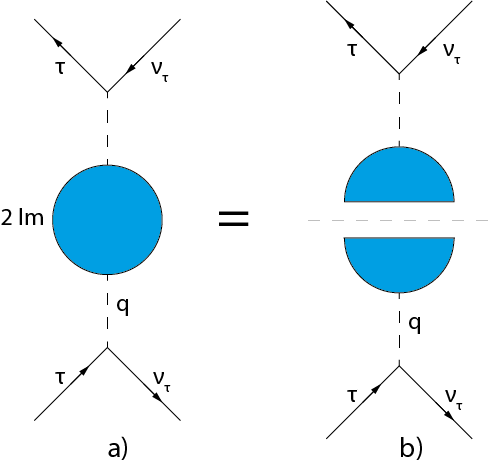
\includegraphics[width=0.6\textwidth]{img/appendix/tauOpticalTheorem.png}
	\caption{The optical theorem relates the imaginary part of a) to the the hadronic $\tau$ decay b). The blue areas, indicate higher order interactions.}
\end{figure}

Starting with the diagrammatical evaluation of Fig. \ref{fig:tauOpticalTheorem} a), making use of of the Feynman rules, we get
\begin{equation}
	\label{eq:tauOpticalAmplitude}
	\begin{split}
		i \mathcal{M} &= (-i)^2 \frac{g^2}{2} \bar u(p_\tau) \gamma_\nu \left(\frac{1-\gamma^5}{2}\right) u(p_{\nu_\tau}) \frac{-i}{M_W^2} \left(\frac{i}{4}\frac{g^2}{2} \Pi^{\mu\nu}(q)\right) \\
		&\times \frac{-i}{M_W^2} \bar(p_{\nu_\tau}) \gamma_\nu \left( \frac{1-\gamma^5}{2} \right) u(p_\tau).
	\end{split}
\end{equation}
Focusing on the spinors, while summing over the spins we can evaluate the traces
\begin{align}
		&\frac{1}{2} \sum_{spins} \bar u (p_\tau) \gamma_\mu \left(\frac{1-\gamma^5}{2}\right) u(p_{\nu_\tau}) \bar u(p_{\nu_\tau}) \gamma_\nu \left(\frac{1-\gamma^5}{2}\right) u(p_\tau) \\
		=\quad& \frac{1}{2} \Tr \left[ \slashed p_\tau \gamma_\mu \left(\frac{1-\gamma^5}{2} \right) \slashed p_{\nu_\tau} \gamma_\nu \left(\frac{1-\gamma^5}{2} \right) \right]\\
		=\quad&\frac{1}{2} \Tr \left[ \slashed p_\tau \gamma_\mu \slashed p_{\nu_\tau} \gamma_\nu \left( \frac{1 - \gamma^5}{2} \right) \right] \\
		=\quad & (p^\mu_\tau p_{\nu_\tau}^\nu + p_\tau^\nu p_{\nu_\tau}^\mu - g^{\mu\nu} p_{\nu_\tau} \dot p_\tau - i \epsilon^{\alpha\mu\beta\nu}p_{\tau, \alpha} p_{{\nu_\tau}, \beta} ),
\end{align}
which then have to be dotted into \eqref{eq:tauOpticalAmplitude}. We notice that $\epsilon^{\alpha\mu\beta\nu} p_{\tau, \alpha} p_{\nu, \beta}$ drops out due to symmetry. We will start regarding only the transversal contribution of the Lorentz-decomposed QCD correlator \eqref{eq:appTauLorentzDecomposition} and later infer the missing longitudinal one. Thus we obtain
\begin{equation}
	\label{eq:appTauAmplitude1}
	\begin{split}
		\frac{1}{2} \sum_{spins} | \mathcal{M}|^2 &= \frac{g^4}{16 M_W^2}(p_\tau^\mu p_\nu^\nu + p_\tau^\nu p_\nu^\mu - g^{\mu\nu} p_\nu p_\tau) (q_\mu q_\nu - q^2 g_{\mu\nu} ) \Pi^{(T)}(q^2) \\
		&=  \frac{g^4}{16 M_W^2} \left[2(p_\tau \cdot q) (p_\nu \cdot q) + (p_\nu \cdot p_\tau) q^2\right] \Pi^{(T)}(q^2).
	\end{split}
\end{equation}
In the center of mass frame we then can find the needed kinematic expressions
\begin{align}
	2 p_\tau \cdot p_\nu = 2 p_\nu \cdot q = M^2_\tau - s \\
	2 p_\tau \cdot q = M_\tau^2 + s
\end{align}
and get the full expression of the transversal amplitude
\begin{equation}
	\begin{split}
		&\frac{g^4}{16 M_W^2} \frac{1}{2} \left[(M_\tau^2 + s)(M_\tau^2 -s) + (M_\tau^2-s)s\right] \Pi^{(T)} (q^2) \\
		=\quad& \frac{g^4}{16 M_W^4} \left[\left(1-\frac{s}{M_\tau^2}\right)\left(1+\frac{2s}{M_\tau^2}\right)\right] \Im \Pi^{(T)}(q^2).
	\end{split}
\end{equation}
Noting from \eqref{eq:appTauAmplitude1} and \eqref{eq:appTauLorentzDecomposition} that the longitudinal contribution differs only by a missing summand $-q^2 g_{\mu\nu}$ we can infer the longitudinal amplitude
\begin{equation}
	\begin{split}
	&\frac{g^4}{16 M_W^4} (p_\tau^\mu p_\nu^\nu + p_\tau^\nu p_\nu^\mu - g^{\mu\nu} p_\nu p_\tau)(q_\mu q_\nu \Pi^{(L)}(q^2)) \\
	 =\quad & \frac{g^4}{16 M_W^4} [ 2 (p_\tau \cdot q)(p_\nu \cdot q) - (p_\nu \cdot p_\tau)s ] \Pi^{(L)}(s) \\
	 =\quad & \frac{g^4}{16 M_W^4} \left[ M_\tau^4 \left(1 - \frac{s}{M_\tau} \right) \right] \Pi^{(L)}(s)
	\end{split}.
\end{equation}
To get to the inklusive hadron decay we have to deal with the integration
\begin{equation}
	\int \frac{\Diff{3} p_{\nu}}{(2\pi)^3} \frac{1}{2E_{\nu}}.
\end{equation}
Due to the massless $\tau$-neutrino and the kinematics we notice that 
\begin{equation}
	|p_\nu| = \frac{1}{2} \frac{M_\tau^2-s}{M_\tau} \quad \text{and} \quad E_\nu = p_\nu
\end{equation}
so that the new integrand can be written as: $\diff p = - \frac{\diff s}{2 M_\tau}$. Thus we get a factor of
\begin{equation}
	\begin{split}
		\int \frac{\Diff{3} p_{\nu}}{(2\pi)^3} \frac{1}{2E_{\nu}} &= -\int \frac{\diff \theta \diff \phi \diff s}{(2\pi)^3} \frac{1}{2 M_\tau} \frac{p_\nu^2}{2 p_\nu} \sin^2 \theta \\
		&= - \int \frac{\diff \Omega}{(2\pi)^3} \frac{\diff s}{4 \dot 2} \left(\frac{M_\tau^2 - s}{M_\tau^2}\right) \\
		&= \int_0^{M_\tau^2} \frac{4\pi M_\tau^2 \diff s}{(2 \pi)^3 8} \left( 1 - \frac{s}{M_\tau} \right)
	\end{split}.
\end{equation}
for the integration part of the $\tau$-decay rate. Now we just have to combine the longitudinal and transversal contribution with the before evaluated integration factor yielding the final decay rate:
\begin{equation}
	\begin{split}
		\Gamma(\tau\to hadrons) &= \frac{1}{2 M_\tau} \int_0^{M_\tau^2} \frac{g^4 M_\tau^6}{M_\tau^2 2^8 \pi^2 M_W^4} \left(1-\frac{s}{M_\tau^2}\right)^2 \\
		& \times \left[ \left(1 + 2 \frac{s}{M_\tau}\right) \Im \Pi^{(T)}(s) + \Im \Pi^{(L)}(s) \right].
	\end{split}
\end{equation}
The $\tau$ decay rate into electron-neutrinos is
\begin{equation}
	\Gamma(\tau\to e \nu_\tau \bar \nu_e ) = \frac{G_F^2 M_\tau^5}{192 \pi^3} = \frac{g^4 M_\tau^5}{32 \dot 192 M_W^4 \pi^3},
\end{equation}
so that the desired ratio is given by
\begin{equation}
		R_\tau = 12 \pi \int_0^{M_\tau^2} \frac{\diff s}{M_\tau^2} \left(1-\frac{s}{M_\tau^2}\right) \left[(1+2 \frac{s}		{M_\tau^2}\Im \Pi^{(T)}(s) + \Im\Pi^{(L)}(s) \right]
\end{equation}	


\section{Coefficients}
\label{app:coefficients}
Taken from \cite{Diogo2011} \\

\subsection{$\beta$ function}
\begin{equation}
	\begin{split}
		\beta_1 &= \frac{1}{6} (11 N_c - 2 N_f), \quad \beta_2 = \frac{1}{12} ( 17 N_c^2 - 5 N_c N_f - 3 C_f N_f), \\
		\beta_3 &= \frac{1}{32} \left(\frac{2857}{54} N_c^3 - \frac{1415}{54} N_c^2 N_f + \frac{79}{54} N_c N_f^2 - \frac{205}{18} N_c C_f N_f + \frac{11}{9} C_f N_f^2 + C_f^2 N_f \right), \\
		\beta_4 &= \frac{140599}{2304} + \frac{445}{16}\zeta(3),
	\end{split}
\end{equation}	
with $C_f = (N_c^2 - 1)/2N_c$.

\subsection{$\gamma$-function}
\begin{equation}
	\begin{split}
		\gamma_1 &= \frac{3}{2} C_f, \quad \gamma_2 = \frac{C_f}{48} (97 N_c + 9 C_f - 10 N_f), \\
		\gamma_3 &= \frac{C_f}{32} \left[\frac{11413}{108}N_c^2 - \frac{129}{4} N_c C_f - \left(\frac{278}{27} + 24 \zeta(3) \right) N_c N_f + \frac{129}{2} C_f^2 \right. \\
		&\left.- \left(23 - 24 \zeta(3)  \right) C_f N_f - \frac{35}{27}N_f^2\right], \\
		\gamma_4 &= \frac{2977517}{20736}-\frac{9295}{216}\zeta(3) + \frac{135}{8} \zeta(4) - \frac{125}{6}\zeta(5).
	\end{split}
\end{equation}	

\subsection{Adler function}
\begin{equation}
	\begin{split}
		c_{11} &= 1, \quad c_{21} = \frac{365}{24} - 11 \zeta_3 - \left(\frac{11}{12} - \frac{2}{3}\zeta(3) \right) N_f = 1.640, \\
		c_{31} &= \frac{87029}{288} - \frac{1103}{4} \zeta_3 + \frac{275}{6} \zeta_5 \\
		& - \left(\frac{7847}{216} - \frac{262}{9} \zeta_3 + \frac{25}{9}\zeta_5 \right) N_f + \left( \frac{151}{162} - \frac{19}{27} \zeta_3 \right) N_f^2 = 6.371, \\
		c_{41} &= \frac{78631453}{20736} - \frac{1704247}{432} \zeta_3 + \frac{4185}{8} \zeta_3^2 + \frac{34165}{96} \zeta_5 - \frac{1995}{16} \zeta_7 = 49.076
	\end{split}
\end{equation}
from \cite{Jamin2006}
\begin{equation}
	\begin{split}
		c_{23} &= 0, \quad c_{22} = \frac{\beta_1 c_{11}}{4}, \\
		c_{34} &= 0, \quad c_{33} = \frac{\beta_1^2}{12} c_{11}, \quad c_{32} = -\frac{1}{4}(\beta_2 c_{11} +  2 \beta_1 c_{21} ), \\
		c_{42} &= -\frac{1}{4} (\beta c_{11} + 2 \beta_2 c_{21} + 3 \beta_1 c_{31}).
	\end{split}
\end{equation}

		
	
		

		
		
\section{Numerical Analysis}
\cite{Chapra2010} \cite{Press2007}
\subsection{Newton-Raphson Method}
\subsection{Newton-Cotes}
\subsection{Gauss Quadrature}

\subsection{Discrepancies between Matthias and my Code}
\begin{itemize}
	\item My spectral moments are slightly lower than Matthias ones (of order $10^{-2}$). Could be caused by the different treatment of weight functions. Mine are integrated with Gaussian Quadratures. Matthias are taken at the center and multiplicated with the bin witdth.
\end{itemize}


% Bibliography:
\bibliographystyle{plain}
\bibliography{references} 

\end{document}


